\documentclass{article}
\usepackage[utf8]{inputenc}
\usepackage{graphicx}

\author{Austin Johnson \\
\texttt{ajohns20@uccs.edu}
\and 
Thomas Mcdonald \\
\texttt{tmcdonal@uccs.edu}
\and 
Hunt Waggoner\\
\texttt{hwaggone@uccs.edu}
}

\title{Targeted Ads from Search Engines}
\date{April 2019}


\usepackage{multicol}



\setlength{\parskip}{1em}

\begin{document}
\maketitle


\section{Abstract}
\textit{
\qquad With many different Search engines available to browse the modern day internet, we show the difference in tracking done by the search engines and how they show targeted advertisement based on what was searched for by the user. We typed in different key words to a search engine and recorded whether the keywords showed up in advertisements. Through this, we were able to track how many searches were queried before the ads appeared. We found that the search engine DuckDuckGo had the least amount of advertisement shown for the keywords entered. }    

\section{Introduction}
\large

\qquad Search engines have always been an integral part of the web. The computer revolution would've never happened if not for yahoo's innovative way of scraping the web for relevant information. Since those days, however, the web has become increasingly more personalized depending on the individual. Our search engine results and advertisements are a prime example of the internet tracking and controlling user experiences. The outrageous amount of data tracking spanning across companies gave our team the idea to see if there is a correlation between search queries and targeted advertisements. Our initial hypothesis is that google search communicates with google analytics and can cater advertisements relevant to what the user has frequently searched. To further our study, we are also going to analyze whether other search engines share information with advertisement software.  


\section{Design}
\large
\qquad For the design of our experiment, we decided scripting our search results would be the fastest and best way to get targeted advertisements. To conduct the experiment, we set up a virtual machine with a fresh install of the latest stable release of Mozilla FireFox. This was done to remove all possibility of previous searches potentially influencing the shown advertisements. Additionally, no ad blockers of any sort were used throughout the course of this experiment.  For the execution of the experiment, we created a list of eleven different key words that were to be used as search parameters in a specific search engine. Our script then opened 50 new tabs with the search results of each key word. To conclude our experiment, we use a list of common websites that are known to be heavily populated with advertisements and see how many targeted advertisements are correlated with our past search queries. 

\textbf{\centerline{Keywords}}
{\centering
\begin{tabular}{ c c c }
    \\
	
	\hline
	
	Tide Pods     & Mercedes Benz            & Apple Watch \\ 
	Dell Computer & Bose Headphones          & Stride Gum  \\  
	Colt AR15     & American Spirits         & Sunglasses  \\
	Condoms       & Colorado Springs Roofing &             \\
	
	\hline
	\\
\end{tabular}
}

For this experiment we decided to use four different search engines to see how how they differed in key word input tracking. With hopes of finding the best search engine for respecting user privacy in their searches. We used :

\textbf{Google -} Google, being the most widely used modern search engine, was the basis for this experiment. With the goal of finding how extensive the user input tracking is for the Google search engine.

\textbf{Bing -} With Bing being owned by Microsoft it was also an option to see if another massive company is conducting a similar amount of tracking as the Google search engine is reportedly on its users.

\textbf{Yahoo -} One of the oldest search engines around, not the most used in the modern day, but with a moderate amount of users Yahoo is still a candidate to see the extent of user input tracking.

\textbf{DuckDuckGo - } The newest of all the browsers we conducted this experiment on, the publishers of this search engine cite on their web page that their number one concern with is to respect user privacy with little to no tracking done on keywords and browsing patterns. As well as stating that they never store any personal data on the user.

	We used our template script, then  changed the url to the search engine we were testing. See the figure below (screencap of code in mintos). After running the script, we went to ten different websites that are known to have a lot of targeted advertisements. The list of websites is:

\textit{
	\begin{itemize}
		\item https://www.theverge.com/
		\item https://www.foxnews.com/
		\item https://www.gamespot.com/
		\item https://stackoverflow.com/
		\item https://www.reddit.com/
		\item https://www.youtube.com/
		\item https://imgur.com/
		\item https://www.amazon.com/
		\item https://www.buzzfeed.com/
		\item https://www.ign.com/
	\end{itemize}
}
	We then visited each site on our virtual box and tallied which websites had a relevant advertisement to our search results. The results for each search engine differ.

\section{Evaluation}
\large
    After conducting our experiments, there was a clear distinction shown between the different search engines. This is highlighted in figure 1. There was a clear difference between the Google search engine and the rest of them. Highlighting the fact that Google uses users inputs to manufacture targeted ads to influence the user. While two of the other search engines Bing and Yahoo still had some user input tracking it was not nearly as severe as Google's tracking.
\begin{figure}[h]
  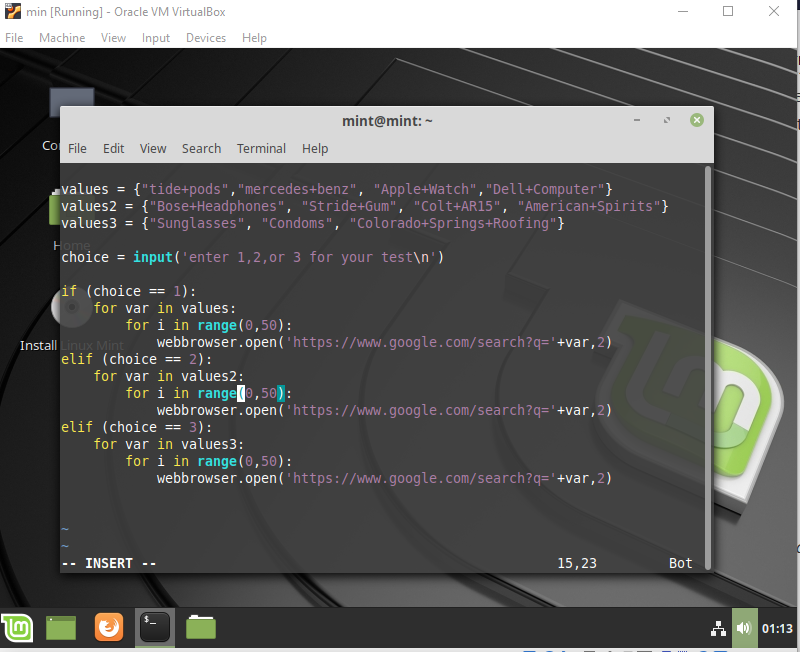
\includegraphics{pic.png}
  \caption{Results}
  \label{fig:boat1}
\end{figure}

Most notably from these results is the DuckDuckGo result. Where the experiment returned zero ads from the keywords, proving that the creators of DuckDuckGo are true to their word in not tracking or storing any user data from their search history. We recommend the use of DuckDuckGo for browsing the internet as a search engine for the user that is wanting to stay anonymous and protect their personal search history. 



\section{Conclusion}

  In the modern world of the internet, and the complex search engines we all use to traverse the internet, input tracking has become a serious user privacy issue. Our experiment found that all three of the biggest search engines by user base track users inputs to target advertisements at their users. The only exception to this was the search engine DuckDuckGo which cites that they do not track or store any user data for any reason. This browser is an acceptable alternative for any user that is worried about protecting their privacy while traversing the internet. 
\end{document}